\section{Проектирование программного средства}
\label{sec:design:intro}

\subsection{Архитектура микросервисов}
\label{sub:design:micro}

Так как разрабатываемая система должна быть легко расширяема для нового функционала и интеграции, быть высокопроизводительной, отказоустойчивой и приспособлена к работе с большим количеством поступающих данных, то в качестве основной модели положенной в разработку данного программного средства была выбрана микросервисная архитектура.

Архитектурный стиль микросервисов -- это подход, при котором единое приложение строится как набор небольших сервисов, каждый из которых работает в собственном процессе и коммуницирует с остальными используя легковесные механизмы, как правило HTTP. 

На рисунке~\ref{fig:micro-vs-mono} представлено сравнение микросервисной архитектуры с монолитной.

\begin{figure}[ht]
\centering
  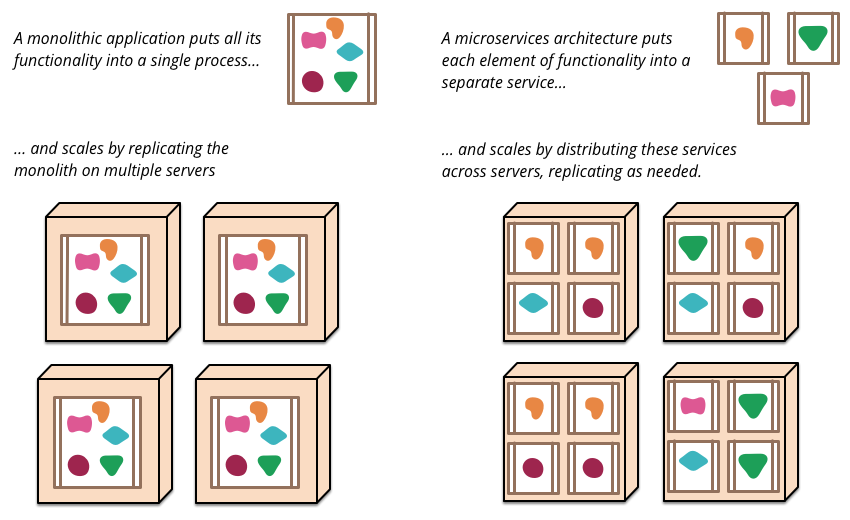
\includegraphics[scale=0.5]{micro-vs-mono.png}  
  \caption{Сравнение микросервисной архитектуры с монолитной}
	\label{fig:micro-vs-mono}
\end{figure} 


Эти сервисы построены вокруг бизнес-потребностей и развертываются независимо с использованием полностью автоматизированной среды. Существует абсолютный минимум централизованного управления этими сервисами. Сами по себе эти сервисы могут быть написаны на разных языках и использовать разные технологии хранения данных. Таким образом система получается легко расширяема для нового функционала и интеграций.

Благодаря тому, что в микросервисной архитектуре легко горизонтально масштабировать отдельные сервисы, её можно приспосабливать к работе с большим количеством поступающих входных данных и добиться высокой производительности.

В то время как монолитные приложения склонны к использованию единственной БД для хранения данных, компании часто предпочитают использовать единую БД для целого набора приложений. Такие решения, как правило, вызваны моделью лицензирования баз данных. Микросервисы предпочитают давать возможность каждому сервису управлять собственной базой данных: как создавать отдельные экземпляры общей для компании СУБД, так и использовать нестандартные виды баз данных. Этот подход называется Polyglot Persistence ~\cite{micro}.

На рисунке~\ref{fig:micro-db} представлено сравнение хранения данных микросервисной архитектуры с монолитной.

\begin{figure}[ht]
\centering
  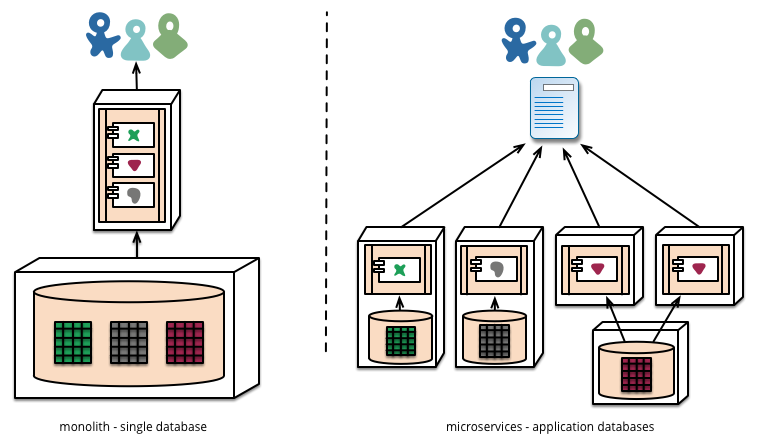
\includegraphics[scale=0.5]{micro-db.png}  
  \caption{Сравнение хранения данных в микросервисной архитектуре с монолитной}
	\label{fig:micro-db}
\end{figure} 



Микросервисная архитектура делает большой акцент на мониторинге приложения в режиме реального времени, проверке как технических элементов (например, как много запросов в секунду получает база данных), так и бизнес-метрик (например, как много заказов в минуту получает приложение). Семантический мониторинг может предоставить систему раннего предупреждения проблемных ситуаций, позволяя команде разработке подключиться к исследованию проблемы на самых ранних стадиях. Таким образом, можно добиваться отказоустойчивости ~\cite{micro}.

Микросервисная архитектура позволяет упростить и ускорить процесс релиза, так как не требует пересборки и развертывания всего приложения, как в случае с монолитным приложением. Вместо этого нужно развернуть (redeploy) только те сервисы, которые изменились.



\subsection{Архитектура программного средства}
\label{sub:design:ps}


Диаграмма взаимодействия сервисов разрабатываемого программного средства представлена на (рисунок~\ref{fig:uc-services}). Актером в данном случае является отдельный микросервис системы, имеющий свою роль в системе. Прецедент – эллипс с надписью, обозначающие какие функции предоставляет тот или иной микросервис.

\begin{figure}[ht]
\centering
  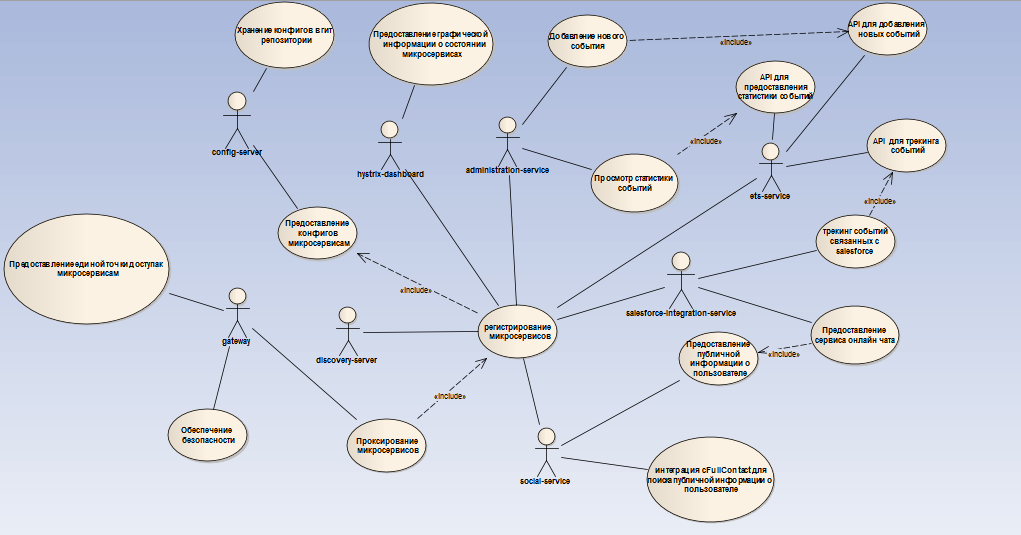
\includegraphics[scale=0.6]{uc-services.png}  
  \caption{Диаграмма взаимодействия сервисов}
	\label{fig:uc-services}
\end{figure} 

На основании представленной диаграммы взаимодействия сервисов можно сделать вывод, что в системе будет существовать семь микросервисов:
\begin{itemize}
\item gateway;
\item config-server;
\item discovery-server;
\item administration-service;
\item salesforce-integration-service;
\item social-service;
\item ets-service.
\end{itemize}
 
Рассмотрим каждого актера с его функциями более подробно:

Discovery-server -- этот сервис позволяет микросервисам обнаруживать друг друга и общаться между собой.

Ets-service -- основной сервис в котором реализовано ядро с работой над событиями. Оно предоставляет API по созданию различных событий и их отслеживанию.

Administration-client -- сервис для администраторов и менеджеров в нем можно настраивать/редактировать/добавлять новые события, следить за их статистикой как за определенный период так и в режиме онлайн. 

Salesforce-integration -- сервис для интеграции с СRM системой Salesforce. Он также предоставляет онлайн чат для клиентов по различным условиям настраиваемым в Salesforce, а также записывает все необходимые события происходящие с CRM Salesforce c помощью ets-service.

Social-integration -- сервис для собирания публичной информации о пользователе, включает в себя интеграцию с FullContact который помогает в сборе информации из доступных социальных сетей, фотографий, географического положения, карьере и около 100 других различных данных о пользователе

Config-server -- это сервис для централизованного хранения конфигурации всех микросервисов в отдельном git репозитории ~\cite{cloud_config}.

Hystrix-dashboard -- это сервис предоставляет возможность графического мониторинга состояния всех микросервисов.

Gateway -- сервис предоставляющий централизованную точку доступа к другим сервисам, а также обеспечивает безопасность для всех остальных сервисов.

\subsubsection{Проектирование системы отслеживания событий}

Данное программное средство позволяет отслеживать события производящие на сайте пользователем. Для того, чтобы система сохраняла только нужные события, она должна позволять настраивать модели событий (удалять/добавлять/редактировать), которые будет способна обрабатывать. При сохранении события система проверяет находится ли подходящая модель для произошедшего события, и если таковая нашлась, сохраняет его.


На рисунке~\ref{fig:des-ets} приведена схема проектирования системы отслеживания событий.
\pagebreak
\begin{figure}[ht]
\centering
  \includegraphics[scale=0.6]{ets.png}  
  \caption{Схема проектирование системы отслеживания событий}
	\label{fig:des-ets}
\end{figure} 	


\subsubsection{Проектирование онлайн чата}
\label{sub:design:chat}

Для понимания того, какие проблемы могут возникнуть у пользователей на сайте будет разработан онлайн чат пользователя с агентом на основе Salesforce Online Chat. Salesforce Online Chat уже изначально включает в себя множество настроек, по которым пользователю будет показано приглашение посетить online chat с тем или иным типом агентом. Данное же программное средство включает в себя доработку возможности настраивать в salesfoce различные чаты для различных страниц сайта клиента. Также перед тем как будет установлен чат, система попробует найти публичную информацию о посетителе и предоставить её агенту, чтобы тот смог её использовать в своих целях (рисунок~\ref{fig:des-chat}).

На рисунке~\ref{fig:des-chat} приведена схема проектирования online chat с пользователем.


\begin{figure}[ht]
\centering
  \includegraphics[scale=0.6]{chat.png}  
  \caption{Схема проектирование Online Chat с пользователем}
	\label{fig:des-chat}
\end{figure} 


